\begin{abstract}

We present a HTTP-based protocol called SASHA; a hybrid approach to home automation, with a focus on privacy and security. Communication is done mostly peer-to-peer, while configuration and management is done is done in a client/server manner. The system automatically and gracefully handles failures in units and network.

\end{abstract}

\section{Introduction}

\subsection{Terminology}
Partitioning in this document should be interpreted as for distributed systems, where it refers to a units being separated due to network failure. When we talk about HTTP we mean HTTP over TLS (HTTPS). An association is a mapping between two units, that only one of the units are aware of. A unit refers to any IP-connected device running SASHA-compliant code.

\subsection{Overview}
SASHA is a partition-tolerant, secure system for home automation over HTTP. New units can be added to the network by swiping it close to the "master" over NFC or other near-field network technology to acquire the networks domain and URLs. The unit then has to be approved by an end-user before access to other units is granted. Authentication is done using a PKI, with certificates being signed by the local master. The system handles dynamic IP allocation by the master keeping an up-to-date mapping between certificates and last seen IP for that certificate. Most communication between units is done peer-to-peer, the master is only involved for handling configuration changes and environment updates, or if a reported sensor value breaches a threshold for something to be done.

Environment changes are notified in real-time to the relevant units from the master, and could be extended to also notify units returning from extended absence about changes since last check-in.

\section{Design and Functionality}

SASHA has two different types of units. In the core there is the master, which keeps track of the other devices in the system. All units in the system is expected to be openly accessible from the Internet. The master is identified by its hostname, which might have a dynamically updated DNS record as its IP changes. The master is the central point of authentication, configuration and management of the units in the network, maintaining a registry of all authenticated units. The master exposes its functionality to the end user through a password-access limited web interface.

The second type of units in SASHA are devices such as sensors and actuators. The relationship between this second type of unit and the master can be described as a client-server relation; the units are initially requesting the master for access to the system, and later performing check-in requests, containing information about their status. The master is collecting and processing this information. The units will check in to the master regularly with status updates. These updates messages serve as a means to get updated sensor data if the unit is a sensor, and to keep the unit's IP address in the registry updated. Additionally they act as a heartbeat, to let the master know when a unit has left the network or been unavailable for a longer period of time, so that the user can be notified and associated units to stop trying to communicate with it.

The connected units are defined by a hierarchy of types. The top level type indicates a set of capabilities that the unit is expected to have. These capabilities are fulfilled in the form of interfaces. Each of these interfaces are again identified by a type which defines the methods they expose, which can be sensor readings communicated during check-ins, or actuators that allow outside sources to instrument the unit to take specific actions, such as turning the light on, start playing a video, or open a door.

\begin{figure}[ht!]
    \centering
    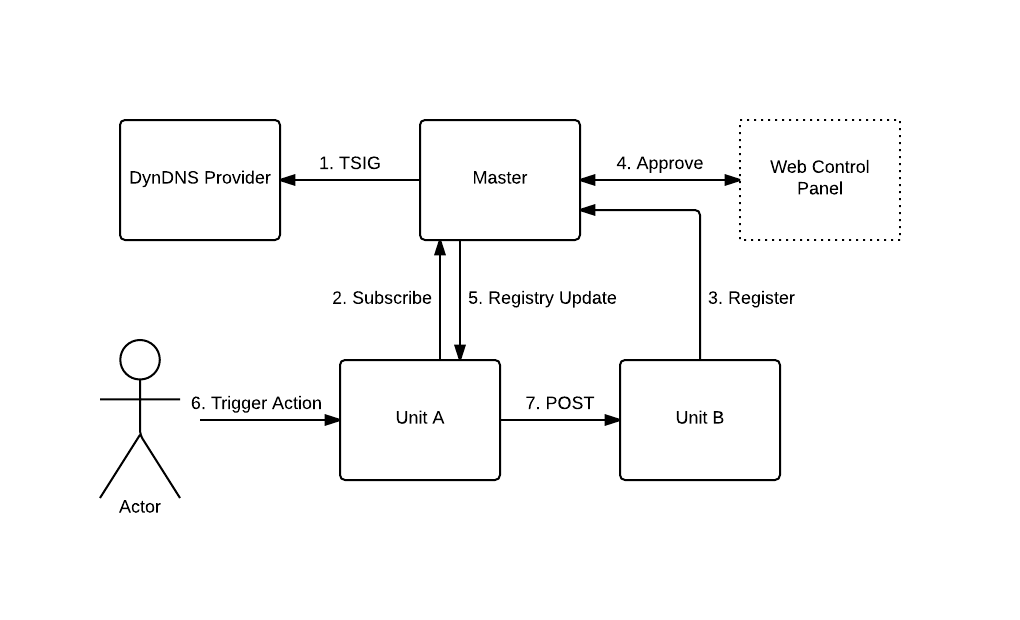
\includegraphics[width=1\textwidth]{subscribe-messaging}\label{fig:subscribe-messaging}
    \caption{SASHA Register Subscribe Pattern. Message \#1 is a DynDNS update record to keep the master hostname updated to the master's current IP. Message number 2 and 3 are both register messages, both only 2 contain subscription information. Message number 7 is a HTTP POST to one of Unit B's interfaces as configured in the master.}
\end{figure}

When all units have been authenticated and associations are set up, there are two forms of communication that will occur, besides the regular check in messages to the master. Something might occur to a unit's physical interfaces, such as motion detected by a camera, buttons being pressed or similar, and the unit will use the data about its associated units as received from the master to instruct them based on the event that occurred. This case is depicted in \autoref{fig:subscribe-messaging}.

In the other case, the master has been configured with a rule, saying that if a given condition occurs, a set of devices should be sent an action, for example if a sensor detects temperatures below a given threshold, send an action to a set of units requesting them to turn on their heating elements.
\section{Self-adaptiveness}
SASHA is self-adaptive, attempting to reduce human intervention to a minimum. This is done through two main strategies, discussed below.

\subsection{Dynamic handling of environment changes}
SASHA thrives in a dynamic system such as IP networks, and sensibly handles offline units and network partitioning. If a unit loses power or network connection, it will automatically restart when power is restored, and automatically inform the master about its restored network status. If the master goes down, all inter-unit communication is unaffected as long as the IPs stay static. Units will continue trying to check-in with the master, with an exponential backoff until it returns.

\subsection{Auto-configuration}
SASHA promotes units to take smart defaults, but always allows the user full control over the interactions. Such defaults might be units subscribing to other classes of units, or to unit tags. This makes sure that newly added light bulbs might be auto-associated to the only light switch in the environment, or that newly added light bulbs tagged with "living room" in the web interface is auto-connected to the light switch in the living room.

When a unit checks in that matches the profile another unit is subscribed to, the other unit will be immediately notified about the new unit and can choose how to react to its presence.

The design is also made so that the user never has to configure anything manually on the device, if the device can perform the swipe with the master, it'll be auto-configured with the masters certificate, necessary URL’s, and will get any other configuration it needs from there, so that the configuration can be auto-applied to several units at once, backed up and restored by the master. This should be a clear usability win for the end user, and might make the devices simpler since they won't need as many inputs for configuration.

\section{Secure Discovery}
\subsection{NFC Swipe Association}
Our design features a secure discovery of new units. The security is based on the idea that each trusted unit will have a certificate signed by the master, which acts as a Certificate Authority. To achieve this, there is a requirement for a trusted channel to communicate the certificate request from a new device to the master. Our proposal for such communication channel is to use a near field communication (NFC) channel, that will allow the new device to send the certificate signing request (CSR) to the master, given that the device is at some point close in proximity to the master. In practice this would require the end-user to “swipe” the new device close to a NFC device associated to the master, to exchange the necessary information to bootstrap the device.

\begin{figure}[ht]
    \centering
    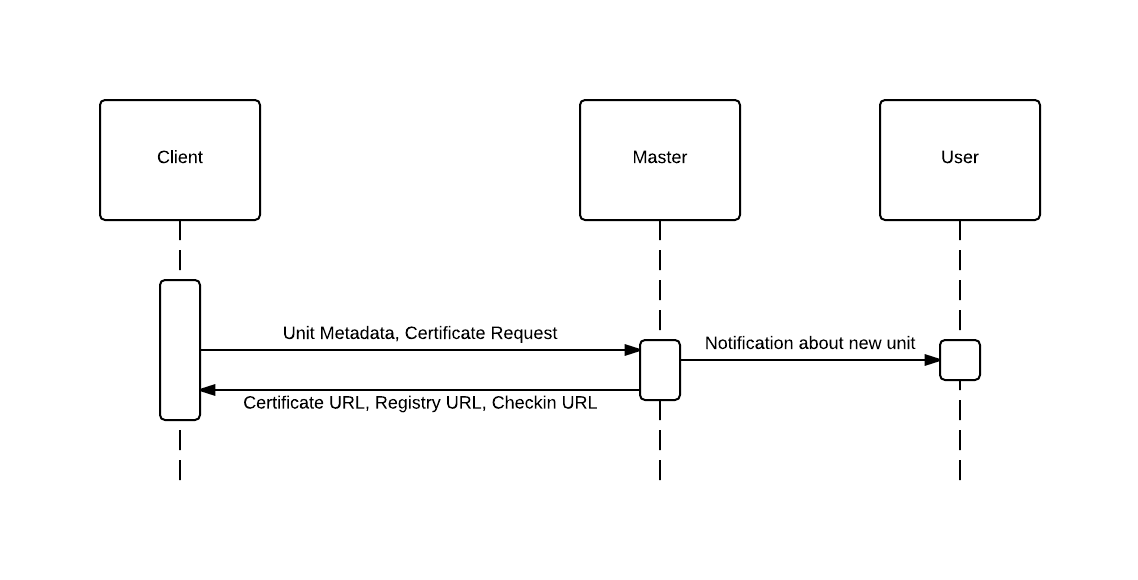
\includegraphics[width=1\textwidth]{swipe}\label{fig:swipe}
    \caption{Messages passed in the Swipe Association Protocol. Note that the new unit will not be able to download its certificate until the user has approved it. After finishing this step, the unit continues with the operations depicted in \autoref{fig:authenticate-unit}.}
\end{figure}

The information exchange over the NFC channel is depicted in \autoref{fig:swipe}. In addition to the CSR required for future secure communication, the new device (client) communicates metadata, such as device type, available interfaces and a textual description of the device. The response is composed of three different URLs to be used by the client as soon as it is connected to the Internet.

\begin{description}
\item[Master certificate]
    The master's TLS certificate.
\item[Certificate URL]
    Says where the unit's signed certificate can be found. This URL will later be used by the client to collect the certificate, which is a requirement to communicate securely all the units in the network.
\item[Checkin URL]
    The checkin URL is used by the client to report to the master, i.e. it allows the client to communicate directly to the master over the Internet through this URL.
\item[Registry URL]
    The registry URL allows the new device to query the registry, i.e. find information about all devices connected to the master. This will allow for more flexibility regarding peer-to-peer communication between devices, as all devices in theory are capable of browsing the entire registry.
\end{description}

After completing the Swipe Association, the new device is awaiting an Internet connection before completing the bootstrap procedure. The master will fully acknowledge the new device when it has performed its first check-in after having been verified by the user, and seeing that the check-in was authenticated with the certificate signed by the master.

\subsection{HTTP Authenticate}
Devices that have gone through the Swipe association will show up in the web interface served by the master, and thus allow the user to verify that the associated devices are indeed intended trusted. The signed certificate will not be generated and made available on the promised Certificate URL until the used manually approves the device through the web interface; requests to this URL will return 404 not found until the user has taken action.
The user have two possibilities; he can reject or approve the device. Approval means that a signed certificate will be made available, thus the device will no longer get a 404, but a 200 OK, and thus complete the bootstrap. Rejection means that requests to the certificate URL will return 410 Gone, thus instructing the device to stop its effort in trying to obtain a certificate, and thus end the bootstrap procedure.

\begin{figure}[ht!]
    \centering
    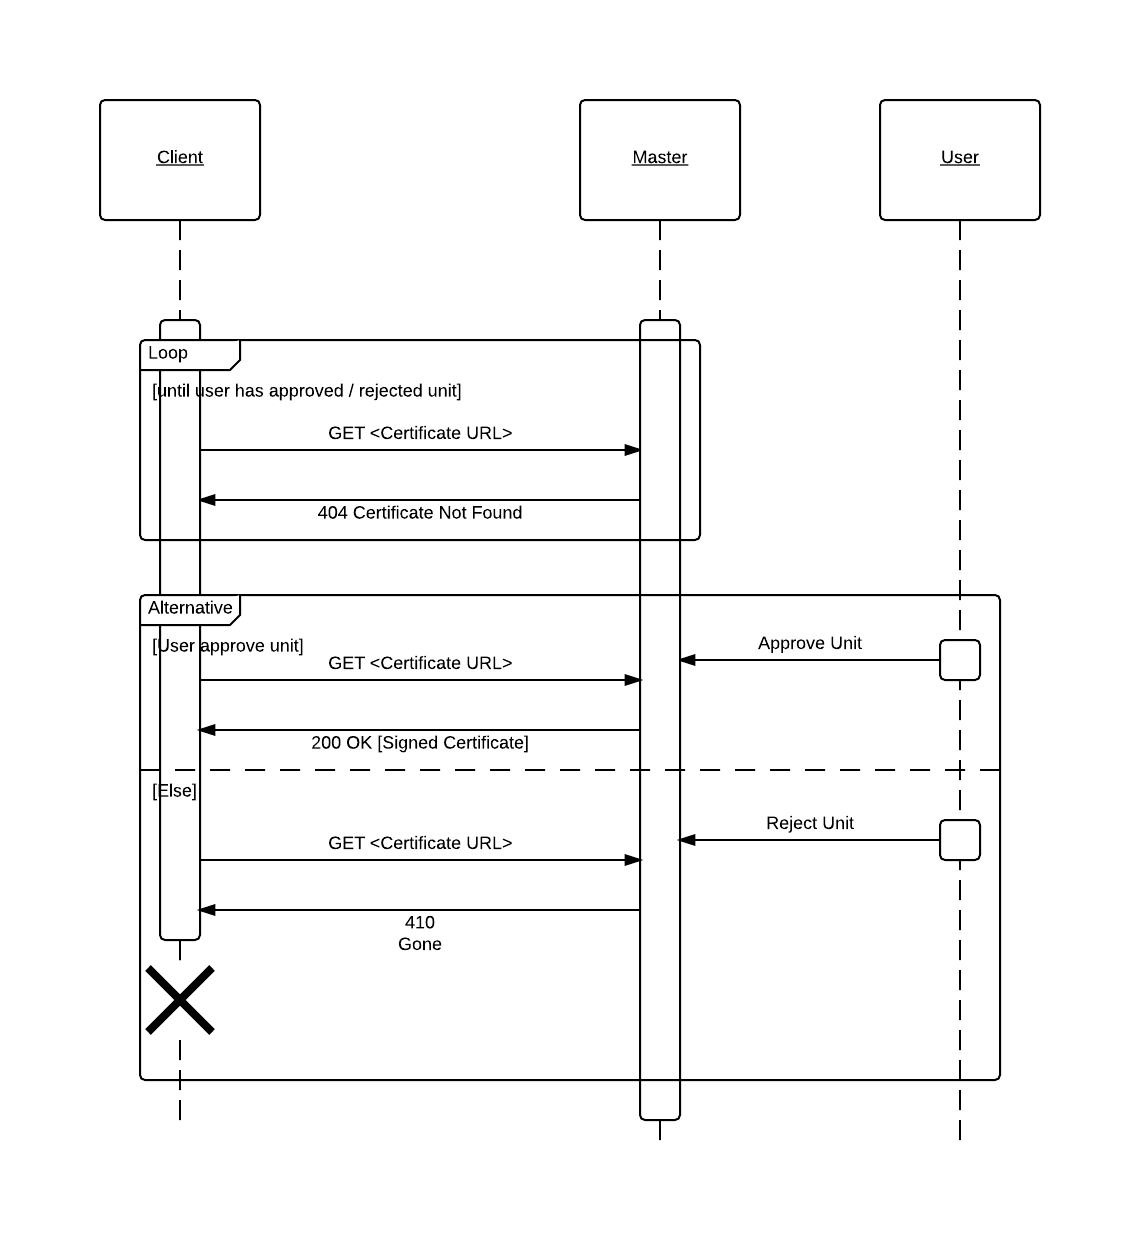
\includegraphics[width=1\textwidth]{authenticate-unit}\label{fig:authenticate-unit}
    \caption{HTTP messages sent during the registration phase. The two cases illustrated are 1) where the user approves the new unit, and 2) the user rejects the new unit.}
\end{figure}

The message flow in these last steps of the bootstrap procedure is given in \autoref{fig:authenticate-unit}. After a successful bootstrap, the device can communicate with the master over a communication channel that provides authentication, confidentiality and integrity.
\section{Justification of Design Choices}

\subsection{HTTP}
The reason for choosing HTTP as our transport protocol boils down to not wanting to reinvent the wheel, when it comes to routing and content negotiation. We utilize the routing features of HTTP to address the different interfaces a unit might provide, and flexible units might use the content-negotiation features provided by HTTP to reply in either JSON, msgpack, XML or others. HTTP also offers content encoding negotiation. Also part of the consideration is framework support, no matter what language you choose to implement your SASHA client in, you'll find several choices for HTTP libraries you might use.

One point about HTTP, and especially HTTP over TLS, is message delay. Many home automation use cases have strict requirements for maximum perceptible delay for the user, f. ex turning on lights. HTTPS requires first a three-way TCP handshake, then a content-negotiation and certificate exchange between communicating parties, before the actual HTTP body can be transmitted. We haven't tested the actual delay you'd get in this setup, but if it turns out to be too large to be practical this could be optimized by the initiating unit always keeping an established TLS connection to associated units, and thus avoiding the handshake phase when data needs to be transmitted. The connections can be established either on first use if there's lots of associated units, or could be established upon the first registry update from the master with the unit's IP if there's few enough associates to keep all the connections around.

\subsection{NFC}
NFC was chosen mostly as an example protocol suitable for close-field communication, since the closeness and direct communication makes it much harder to compromise this channel. If the initial setup was done over the Internet, a clever attacker could perform a Man-in-the-Middle attack on the association, and thus gaining access to your network internals.

\subsection{Security}
We wanted to make the SASHA system secure, because we think it's an essential requirement for any Internet-facing service being developed today. Building the protocol on top of HTTP also helps make this step rather simple, since tools for working with client certificates over HTTPS are well supported. We consider security to be one of the most important challenges in the coming Internet of Things-age, as the number of units connected to the Internet will increase greatly, and thus the consequences of poor security will get even worse than it is today. It is also a privacy concern, household devices work on a lot of sensitive data, such as your habits, preferences, location, and much more, which should remain confidential also in a network of smart units.

No device will be able to access any other before a manual approval has been done through the master web interface. Devices are handed the master's certificate at registration time, and will check each interacting device for a valid certificate signed by the master. The master's certificate is not expected to be signed by any known certificate authority, since the master needs to be able to sign certificates himself. One benefit of this is that the certificates generated can utilize elliptic curve cryptography, which is much faster and better suited for resource constrained units that you might expect to find in a home automation scenario than traditional RSA-based certificates.

\section{DynDNS Provider Market Potential}
Detection of new units in SASHA relies on the master to have a resolvable hostname or a static IP address. Since most households would probably not provide static IP addresses without additional configuration, the static hostnames seem like the most natural design.
The need for resolvable hostnames will allow devices to locate the master despite changing IP addresses. However, this comes with the cost of a new requirement, being a DNS server to keep track of the masters changing IP address.

A dynamic DNS requirement is not something that can be fulfilled by the parts by SASHA alone. This enables manufacturers of SASHA devices, or other third party providers, to provide hostnames as a service, which again potentially can be monetized. This would enable customers to access their master on domains such as myname.sasha.org or similar.

\section{Related Work}

Now we'll discuss some other home automation tools and see how they compare to SASHA.

ZigBee\cite{zigbee} is a wireless mesh network often used for sensors to report in to devices, designed for low-power low-rate communication. ZigBee complements SASHA and could co-exist, as sensors could report in wirelessly to controlling devices, which then reports in to the master. Since the sensors are not on a IP network directly, this poses little to no additional risk.

OSGi\cite{osgi} is a Java-specific framework, which only works on units that can run a Java VM. OSGi also doesn't seem to encrypt communication or ensure the identity of communicating parties, as their security layer only seems to make sure execution is limited to pre-defined modules. SASHA is a network-level standard that can be implemented in any language on any platform.

Z-Wave\cite{z-wave} is another mesh network technology, operating on 900Mhz. Z-Wave does not seem tailored to Internet of Things, where every unit has an IP address. Since Z-Wave doesn't have any central point, there's also no authentication of new devices, so the setup is relatively easy infiltrate for an attacker.

INSTEON is yet another wireless mesh networking technology, which also due to its mesh nature and employs no authentication or end-to-end encryption, and would also be limited to devices in close physical proximity. SASHA is completely independent tn physical proximity and can control any device connected to the Internet, whether in the next room or on a different continent.

The IETF is working on standardizing formats for Internet of Things, one of the formats they're working on, SenML \cite{senml}, is a format for reporting sensor values to other devices. This is quite similar to how our sensors report values to the master, or could perhaps be utilized over ZigBee to have wireless sensors without an IP to report to a connected unit.

In researching the other solutions it appears that many of the units produced today are made to one specific networking technology, which isn't exactly in the Internet spirit of heterogeneous units communicating over lots of different interfaces and technologies. Basing communication to IP networks like SASHA does makes it possible for a device vendor to comply to multiple different standards and not locking the user in to one specific solution. There also seems to be none of the other solutions that take authentication and security seriously, which absolutely should be taken into account with all the sensitive data flowing through a home automation network.

For a more through comparison of INSTEON, Z-Wave and other networking technologies, we refer the reader to the 2010 report by Gomez and Paradells \cite{comparison-of-technologies}.

\section{Security Considerations}

Private keys should be securely stored in the devices, such that it cannot be retrieved by an attacker (which is definitely not the case for our Raspberry Pi environment, where anyone can retrieve the data from the unencrypted memory card).
The swipe is the most critical step in the system, as the NFC channel must be trusted. During the swipe protocol, an attacker can impersonate the initial request, containing the public key (CSR) of a device, thus the attacker can set up a man-in-the-middle attack at this stage.
References
